
\chapter{Conclusion}

In this thesis, we have expanded on recent work on semi-dense visual odometry by exploring means of relocalizing a query camera. We applied existing RGB-D techniques using only RGB and our partial depth data. We also investigated the effectiveness of a learned descriptor in this context. Furthermore, we evaluated our pipeline on two public benchmark datasets, and showed that relocalization using a straightforward application of SIFT features is still viable in this domain. Because the topic of direct visual odometry using semi-dense techniques is relatively new, this explores potential opportunities and pitfalls.

\section{Future Work}

We anticipate that many existing techniques can be further explored in the context of semi-dense depth data.

Firstly, many methods \cite{valentin2015exploiting} \cite{schmidt2017self} have made improvements by reckoning about the uncertainty of their estimates. This can frequently be combined with, for example, the Mahalanobis norm in an iterative refinement step to weight observations according to their certainty. In the case of DSO, where we are seeking to minimize the error of Gaussian-distributed observations, the Hessians of our inverse depth estimates give a measure of the uncertainty. For example, in \fref{fig:uncertainty}, we visualize the variance.

\begin{figure}[h]
	\centering
	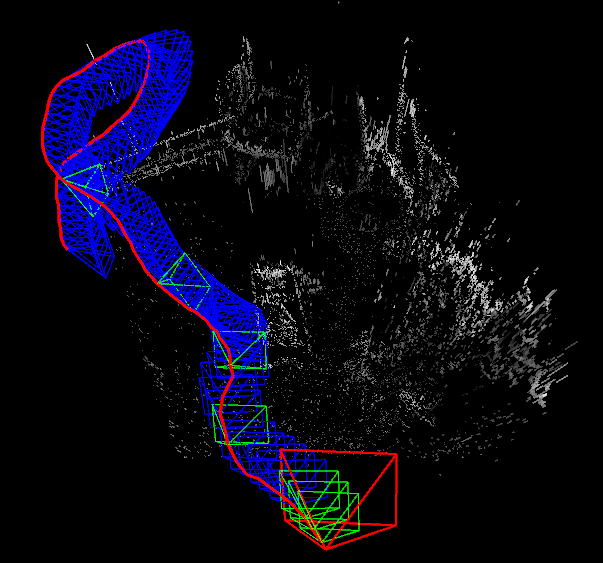
\includegraphics[width=0.4\linewidth]{conclusion/uncertainty.png}
	\caption{DSO at runtime, with only points in the current active window displayed. Active keyframes are marked in green. Here, each point is elongated according to the variance of its inverse depth measurement. As a result, points that are far away or in newly observed areas are stretched out.}
	\label{fig:uncertainty}
\end{figure}

Other approaches also trade accuracy for speed. For example, in small scenes and other scenarios where a camera is likely to revisit the same pose, the randomized ferns approach of \cite{shotton2013scene} would be very effective. These ferns sample random pixels in the RGB-D imagery, so in the case of semi-dense data, one could in-paint the depth or otherwise provide a proxy for the true pixel sample.

Furthermore, since DSO acts on a small window of past keyframes, it would be reasonable to consider windowed temporal data. The authors of VidLoc \cite{clark2017vidloc} do exactly this by training LSTMs on RGB-D video. Additionally, although visual descriptors are generally highly informative, exploring applications of geometric descriptors could be prudent, as in \cite{zeng20163dmatch}, due to the dense, low-drift pointclouds that semi-dense methods generate over time.

For this thesis specifically, we believe that further investigation into failure cases of descriptor matching and pose estimation would be valuable. It also remains to be seen to improve localization for larger scale scenes, and for scenes that are inherently difficult for monocular camera tracking, such as shaky or low frame-rate video. Furthermore, integrating this work directly into a live SLAM pipeline to perform loop closure and recovery from tracking loss would give a complete view of gains that stand to be made.

\cleardoublepage

